\section{Theorie}
\label{sec:Theorie}
Die folgende Theorie ist auf \cite{Anleitung44} basiert.

\subsection{Die Röntgenröhre}
\label{subsec:Röntgenröhre}
In diesem Versuch wird eine Röntgenröhre mit Cu-Anode verwendet. In dieser werden Elektronen aus einer Glühkathode in Richtung Cu-Anode beschleunigt. Die in die Cu-Anode einschlagenden Elektronen interagieren dann mit dem Kupfer, und zwar auf zweierlei Arten: Durch Stöße mit den Elektronen in den Kupferatomen werden diese auf höhere Niveaus angeregt. meistens werden die Atome sogar ionisiert. Dies macht Plätze auf niedrigeren Niveaus frei und führt damit dazu, dass Elektronen höherer Niveaus unter Emission von Röntgenstrahlung auf auf diese niedrigeren Niveaus zurückfallen. Außerdem wird bei der Bewegung der Elektronen im elektrischen Feld innerhalb des Kupfers Bremsstrahlung emittiert.\\
In diesem Versuch wird die $\text{K}_\alpha$-Linie von Kupfer verwendet, also jene Röntgenstrahlung, welche beim Niveauübergang von der zweiten auf die erste Schale entsteht. Sie besitzt eine Wellenlänge von $\lambda=1.54\text{Å}$. Um diese aus dem restlichen Spektrum der Röntgenröhre herauszufiltern, wird ein \textit{Göbelspiegel} verwendet. Dieser bündelt die Strahlung und filtert alle anderen Linien aus der Strahlung heraus.\\
Die Strahlung fällt nach dem Göbelspiegel auf eine Blende, dann auf die Probe und dann auf eine weitere Blende. Die Blenden dienen dazu, den eingestellten Glanzwinkel der einfallenden und den gemessenen Glanzwinkel der ausfallenden Strahlung zu variieren.\\
\\
Bei sehr geringen Winkeln (kleiner als $\alpha_g$) schießt die Strahlung über die Probe hinaus. Dies äußert sich in einem reskalierenden Faktor vor der gemessenen reflektierten Intensität, dem \textit{Geometriefaktor} 
\begin{aquation}
    G &\coloneqq \left\{ \begin{matrix}
        \frac{D \sin{\alpha_i}}{d_0} & \alpha_i < \alpha_g \\
        1 & \text{sonst}
    \end{matrix} \right. \tc
    \label{eq:Geometriefaktor}
\end{aquation}
mit der Probenlänge $D$ und der Strahlbreite $d_0$.

\subsection{Der komplexe Brechungsindex}
Dringt elektromagnetische Strahlung in ein nicht absorbierendes Material ein, so nimmt der Brechungsindex einen reellen Wert an. Die Dispersionsrelation nimmt dann die Form 
\begin{aquation}
    k(\omega) &= \odiv{c}\omega n(\omega)
\end{aquation}
Diese Relation taucht direkt in der ebenen Wellengleichung auf, welche die Form 
\begin{aquation}
    \psi(x,t) &= \psi_0 e^{i( k(\omega) x - \omega t)}
\end{aquation}
annimmt.\\
Anhand dieser Tatsache lässt sich durch einige grundlegende mathematische Überlegungen ableiten, wie die Dispersionsrelation für den Fall eines absorbierenden Materials auszusehen hat. Absorption führt in der Welleenfunktion nämlich bekanntermaßen zu einem komplexen Anteil in der ansonsten reellen Wellenzahl. Dieser Anteil führt in der Wellenfunktion zu einem zusätzlichen Faktor, welcher einer Exponentialfunktion mit reellem negativen Koeffizienten führt, welche wiederum dafür sorgt, dass die Amplitude der Wellenfunktion immer weiter gegen null abflacht.\\
Da die Wellenzahl linear im Brechungsindex ist, liegt es nahe, diesen komplexen Anteil mit in den Brechungsindex aufzunehmen. Der resultierende komplexe Brechungsindex nimmt dann die Form 
\begin{aquation}
    n(\omega) &= \chi+ i \kappa
\end{aquation}
an. Der Absorptionskoeffizient $\kappa$ ist ein Maß für die Abflachung der Wellenfunktion, während $\chi$ der Realteil des Brechungsindex ist.\\
Im Falle von Röntgenstrahlung ist der Realteil des Brechungsindex typischerweise $\chi = 1-\delta$, wobei $\delta$ typischerweise in der Größenordnung $10^{-6}$ liegt. Für diesen Fall, in dem der Realteil kleiner als $1$ ist, existiert ein kritischer Winkeln $\alpha_C$. Für Glanzwinkel $\alpha<\alpha_C$ tritt Totalreflexion auf. Aus dem Brechungsgesetz von Snellius 
\begin{aquation}
\label{eq:brechungsgesetz}
    n_1 \sin(\theta_1) &= n_2 \sin(\theta_2)
\end{aquation}
lässt sich der kritische Winkel als jener Einfallswinkel ableiten, bei welchem der transmittierte Strahl parallel zur Oberfläche verläuft, was dem Setzen von $\theta_2=\frac{\pi}{2}$ entspricht. Der Index $1$ ist dabei f[r Winkel und Brechungsindex vor der Streuung reserviert, während für den Fall danach der Index $2$ verwendet wird.\\
Da im vorliegenden Fall der kritische Winkel für kleine $\delta$ benötigt wird, lässt sich dieser zu 
\begin{aquation}
    \alpha_C &\approx \sqrt{2 \delta} \tp
    \label{eq:alpha_C}
\end{aquation}
Nach der Streuung am Versuchsobjekt zerteilt sich die Welle in eine transmittierte Welle (Label $t$) und eine reflektierte Welle (Label $r$), wodurch sich die Gesamtwelle zu 
\begin{aquation}
    \psi(x,t) &= t \psi_t (x,t) + r \psi_r (x,t) \tp
\end{aquation}
Der Transmissions- und der Reflexionskoeffizient ergeben sich nach den Fresnel-Gleichungen, welche sich aus dem Brechungsgesetz \autoref{eq:brechungsgesetz} ableiten lassen, zu 
\begin{aquation}
    t &= \frac{2 n_1 \sin(\alpha_i)}{n_1\sin(\alpha_i) + n_2\sin(\alpha_t)} \\
    r &= \frac{n_1 \sin(\alpha_i) - n_1 \sin(\alpha_t)}{n_1 \sin(\alpha_i) + n_2 \sin(\alpha_t)}
\end{aquation}

Diese Größen sind jedoch keine direkten Observablen, sondern Wahrscheinlichkeitsamplituden. Die physikalischen Größen sind die \textit{Reflektivität} $R \coloneqq |r|^2$ und die \textit{Transmission} $T \coloneqq |t|^2$.\\
Außerdem sind sie linear abhängig voneinander, verknüft über die Relation $1 = R + T$. Aus diesem Grund genügt es, eine der beiden Größen zu messen. Für den Fall $\alpha_i > 3 \alpha_C$ ergibt sich die Reflektivität zu
\begin{aquation}
    R &= \left(\frac{\alpha_C}{2 \alpha_i}\right) \tp
    \label{eq:Fresnel}
\end{aquation}


\subsection{Effekte in Mehrschichtsystemen}
Unter der Annahme mehrschichtiger Systeme treten weitere Effekte auf. Ihre Ursache liegt darin begründet, dass bei jedem Schichtübergang ein Teil der Welle reflektiert und ein Teil transmittiert wird. Der Gangunterschied zweier Teilwellen resultiert darin, dass diese miteinander interferieren.\\
Konstruktive Interferenz tritt generell immer dann auf, wenn die Welle nicht phasenverschoben ist. Bezüglich des Gangunterschieds bedeutet dies, dass wenn der Gangunterschied insgesamt ein Vielfachte von $\lambda$ ist, konstruktive Interferenz auftritt. Destruktive Interferenz hingegen tritt auf, wenn der Gangunterschied ein ungerades ganzzahliges Vielfaches von $\frac{\lambda}{2}$ ist.\\
In diesem Versuch gibt es nur zwei Schichten. 
Dieses Interferenzverhalten schlägt sich in der Reflektivität nieder. Diese ist proportional zu der in diesem Versuch gemessene Observable der reflektierten Intensität gemäß der Relation 
\begin{aquation}
    R &= \frac{I_\text{r}}{I_\text{tot}}
\end{aquation}
mit der totalen Intensität des emittierten Strahls $I_\text{tot}$. Nach den Gesetzen der Trigonometrie resultiert eine Änderung des Einfallswinkels in einer Änderung des Gangunterschieds. Wird also ein hinreichend großer Winkelbereich abgefahren, sollten mehrere Interferenzmini- und -maxima auftreten. Diese Schwingungen werden \textit{Kiessig-Oszillationen} genannt. Ein Beispielplot f[r diese ist in \autoref{fig:kiessig} zu sehen.
\begin{figure}
    \centering
    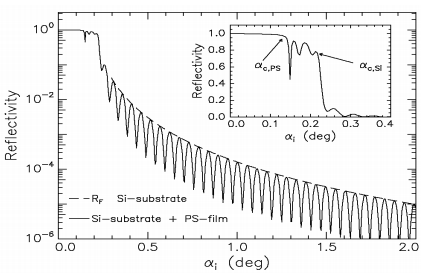
\includegraphics[width=\textwidth]{figures/kiessig.png}
    \caption{Kiessig-Oszillationen für einen Silizium-Wafer mit einer $800\si{\angstrom}$ dicken Polysterol-Schicht.}
    \label{fig:kiessig}
\end{figure} 

\subsection{Bestimmung der Schichtdicke}
Um die Dicke einer einzelnen Schicht zu bestimmen, wird die \textit{Bragg-Bedingung} 
\begin{aquation}
    n\lambda &= 2 d \sin(\alpha_i)
\end{aquation}
verwendet. Diese Gleichung setzt die Schicktdicke in Abhängigkeit des $n$-ten Minimums der Kiessig-Oszillation. Um diesen Parameter loszuwerden, wird die Differenz zwischen den Fällen $n+1$ und $n$ betrachtet. Da die hier verwendeten Glanzwinkel klein sind, kann der Sinus als $\sin(\alpha_i) \approx \alpha_i)$ genähert werden, sodass sich für die Differenz zweier benachbarter Interferenz-Extrema und damit direkt für die Schichtdicke die Formel 
\begin{aquation}
    d = \frac{\lambda}{2 \Delta\alpha_i}
\end{aquation}
ergibt.\\
Im Falle mehrerer Schichten überlagern sich aufgrund der Tatsache, dass es mehr als zwei Schichten gibt, mehrere austretenden Strahlen, welche unterschiedliche Anzahlen von Schichten durchlaufen haben, miteinander. Im Gegensatz dazu gab es bei einer einzelnen Schicht nur zwei Anteile: Den direkt reflektierten und den, welcher die eine Schicht durchlaufen hat.\\
Dies führt dazu, dass sich die Osziellationen aus allen Schichten ergeben, weswegen das Endergebnis nicht mehr direkt mit der Dicke einer einzelnen Schicht verbunden ist. Um die einzelnen Schichtdicken zu bekommen, gibt muss daher der \textit{Parrat-Algorithmus} verwendet werden. Dieser leitet sich her, indem das Amplitudenverhältnis $Q_j \coloneqq \frac{R_j}{T_j} = \frac{R_j}{1-R_j}$ zweier benachbarter Schichten an der $j$-ten Grenzfläche bestimmt wird. Da sich hier nämlich der Anteil der transmittierten Welle direkt von dem der reflektierten Welle ableiten lässt, lässt sich so durch Umstellen aus den Fresnel-Gleichungen direkt die Einfallende Welle für die folgende Grenzfläche bestimmen. Dies führt zu der Rekursionsformel 
\begin{aquation}
    Q_j &= e^{-2 i k_{z,j} z_j}\frac{r_{j,j+1} + Q_j e^{-2 i k_{z,j+1} z_j}}{1 + r_{j,j+1}  Q_j e^{-2 i k_{z,j+1} z_j}} \tc
    \label{eq:Parratt}
\end{aquation}
bei der 
\begin{aquation}
    k_{z,j} &\coloneqq k \sqrt{n_j^2 - \cos^2{\alpha_j}}
\end{aquation}
ist, während 
\begin{aquation}
    r_{j,j+1} &= \frac{k_{z,j} - k_{z,j+1}}{k_{z,j} + k_{z,j+1}}
\end{aquation}
der bereits zuvor definierte, diesmal jedoch durch die Wellenzahlen vor und nach der Streuung an der Grenzfläche ausgedrückt Fresnel-Reflexionskoeffizient, ist.\\
Zur Veranschaulichung der Schichtdurchgänge, welche durch den Parratt-Algorithmus berechnet werden können, dient \autoref{fig:parratt}.

\begin{figure}
    \centering
    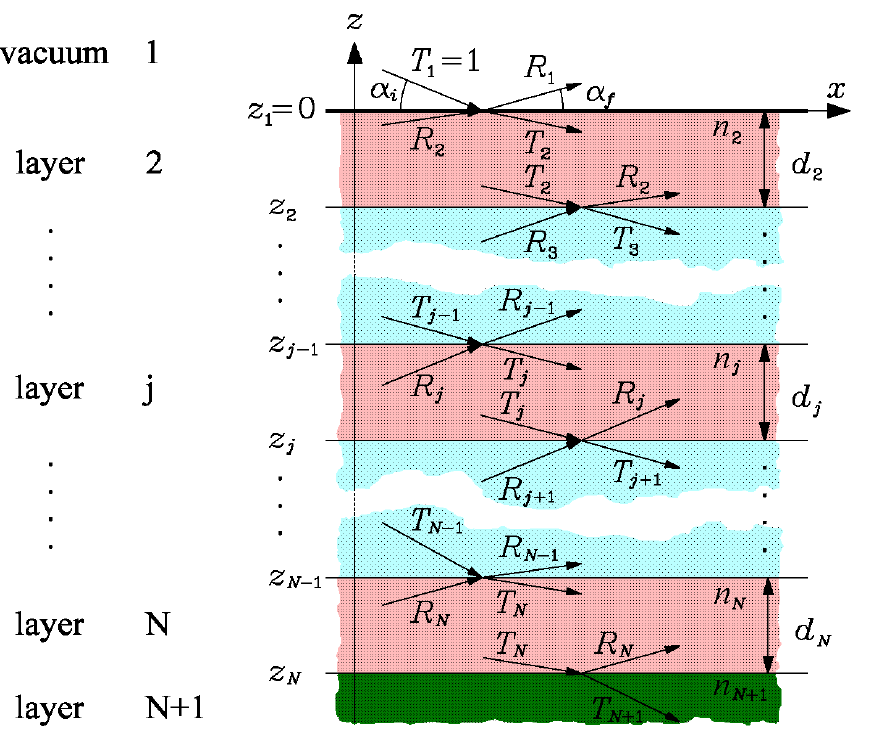
\includegraphics[width=\textwidth]{figures/parratt.png}
    \caption{Veranschaulichung der wiederholten Reflexionen bei mehreren internen Schichtübergängen, welche durch den Parratt-Algorithmus berechnet werden können.}
    \label{fig:parratt}
\end{figure}

\subsection{Messung der Rauigkeit}
Die bisherigen Überlegungen wurden alle unter der Annahme angestellt, dass die einzelnen Oberflächen alle ideal glatt sind. In der Realität besitzen Oberflächen jedoch kleine Unebenheiten, welche sie rau machen. Diese Rauigkeit sorgt für eine Abweichung vom von der Theorie postulierten Endergebnis. Um diese Abweichung zu berücksichtigen, wird eine weitere Größe eingeführt: Die \textit{Rauigkeit}
\begin{aquation}
    \sigma_j^2 &\coloneqq \int dz\left(z - z_j\right)P_j(z) \tp 
\end{aquation}
Dabei sind die $z_j$ die Ortskoordinate der $j$-ten Grenzfläche. Das Wahrscheinlichkeitsmaß $P_j$ ist ein Maß für den Anteil der Fläche, welcher in einem infinitesimalen Intervall um die Koordinate $z+z_j$ liegt. Die Rauigkeit ist also das quadratische Mittel über alle Abweichungen von der perfekten Glätte. Für eine perfekt glatte Fläche verschwindet die Rauigkeit, da hier gilt $P(z) = \delta(z)$, was genau mit der linguistischen Definition der Begriffe \textit{rau} und \textit{glatt} zusammenfällt.\\
Angewandt auf die Fresnel-Koeffizienten führt die Rauigkeit zu einem zusätzlichen Vorfaktor, sodass diese nun die Form 
\begin{aquation}
    \bar{r}_{j,j+1} &\coloneqq r_{j,j+1}\hsf e^{-2 k_{z,j}k_{z,j+1}\sigma_j^2} \\
    \bar{t}_{j,j+1} &\coloneqq t_{j,j+1}\hsf e^{\left( k_{z,j} - k_{z,j+1}\right)^2\frac{\sigma_j^2}{2}}
\end{aquation}
annehmen.\cite{RoughSurfaceReflectometry}
